\chapter{Planteamiento del algoritmo en software}
\section{Recopilacion de los datos}
Para la recopilacion de los datos se utilizara la libreria wfdb que se encarga de proporcionar
funciones para leer y escribir archivos de diferentes formatos que contienen señales biomédicas,
como archivos de registro de señales (por ejemplo, formato .dat), archivos de anotaciones
 (por ejemplo, formato .atr) y archivos de cabecera (por ejemplo, formato .hea).

 Los pacientes vienen identificados por un id (por ejemplo, 101) y hay 3 ficheros por paciente, 
 con extensiones .dat, .atr y .hea

\begin{figure}[h!]
	\centering
	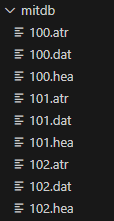
\includegraphics[width=0.2\textwidth]{./Images/img_algoritmo/ficheros_pacientes.png}
	\caption{Ficheros que contienen la señal de cada paciente}
	\label{fig:seniales_pacientes}
\end{figure}

Se descarga la base de datos con la funcion de la libreria de wfdb, dldatabase que recoge 
la señal del paciente y las anotaciones de los cardiologos sobre cada pico QRS.

los pacientes de la base de datos se han hecho una prueba de 30 mins lo que en la señal 
equivale a 650000 samples
